\chapter{应用场景}
\label{chap:application}

在这篇论文中,我们提出了一个针对具有良好格式的日志,以条目为粒度的压缩策略。
传统的压缩策略通常以块为粒度进行压缩和解压缩,和它们相比,我们的策略能够
从中间位置直接解压缩一条记录,而块压缩需要从块的开始位置顺序解压缩,直至
遇到目标条目为止。获取一条日志,块压缩平均下来需要解压半个块的数据,而我们
只需解压缩一条日志,从而节省了解压缩时间和CPU资源。

上述特性使得我们的压缩方法适用于日志分析,在本章中我们将会讨论两个使用我们
压缩策略做日志分析的应用场景。

\begin{figure*}
        \centering
        \subfigure[块为粒度压缩策略]{
                \label{fig:block_level}
                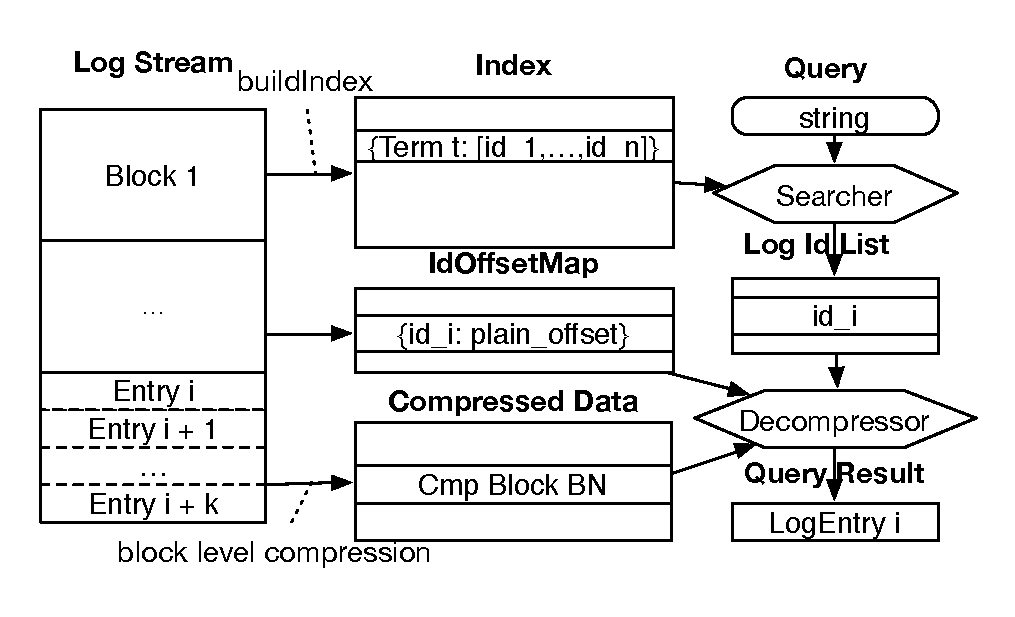
\includegraphics[width=0.8\textwidth]{figures/block_level.eps}
        }
        ~ %add desired spacing between images, e. g. ~, \quad, \qquad, \hfill etc.
          %(or a blank line to force the subfigure onto a new line)
        \subfigure[条目为粒度压缩策略]{
                \label{fig:record_level}
                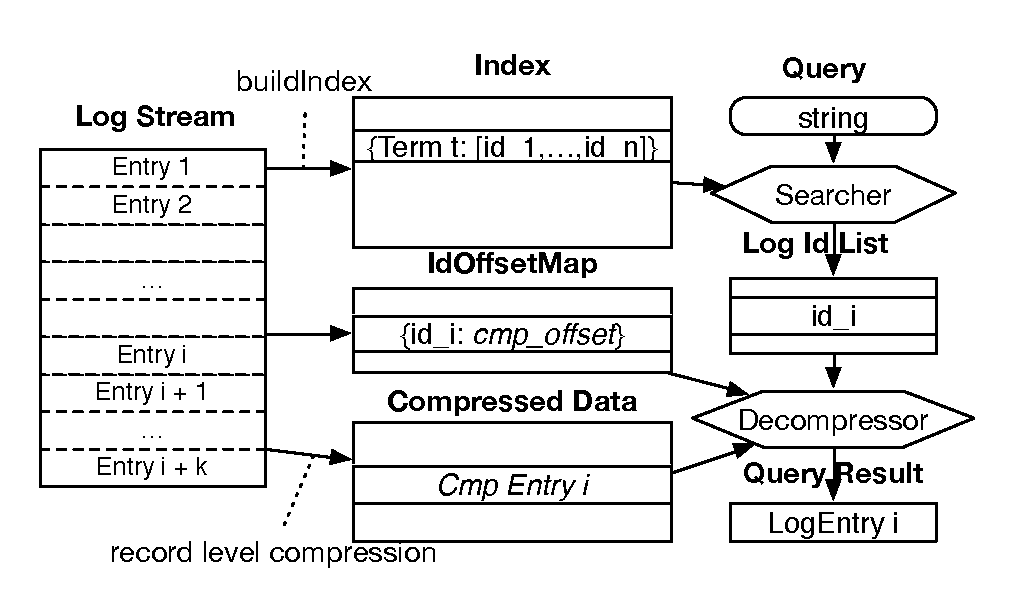
\includegraphics[width=0.8\textwidth]{figures/record_level.eps}
        }
        \caption{比较块为粒度和条目为粒度的压缩策略在对日志建立索引,进行搜索时的不同}
        \label{fig:compare}
\end{figure*}

\section{索引搜索日志}

调试日志一种最简单和最常用的方法是使用``grep''命令去获取一条特定的消息~\cite{Oliner2012}。
然而,这种方法有着许多的限制:1)每次做``grep''操作需要扫描整个文件,而从硬盘读取文件
非常的缓慢。2)它不支持范围查询,并且很难构建复杂的布尔语句查询。
为了解决这两个限制,人们通常采用一个两阶段的策略,即首先对日志文件建立索引,
以后的查询只需查找索引文件即可。
而为了节省硬盘空间,原始日志数据通常会被压缩。

我们在\reffig{compare}说明如何将Cowic整合到日志搜索系统之中。
\reffig{block_level}(a)举例说明了传统的块压缩策略是如何被整合到建立索引和进行查询的过程之中。
首先有一个建立索引的程序,对原始日志建立反向索引,并构建一个ID映射表。
对于每个关键字,反向索引中存储了和这个关键字关联的日志ID的列表,
而ID映射表记录了每个日志ID对应的日志在原始文件中得位置。
原始日志被以块为单位进行切割,然后对每一个块分别进行压缩。
当我们执行一个查询时,我们首先查找反向索引获得结果日志ID的列表,
而从ID映射表中,我们能获取每个ID对应日志的位置,从而计算出包含这个位置的块。
最后,我们解压缩对应的块,从中获取原始日志条目,将最终结果返回给用户。

\reffig{compare}(b)则说明了如何将以条目为粒度的压缩策略整合到上述过程。
我们不需要修改建立索引和查找索引的过程,
唯一的区别是在ID映射表中我们现在存储日志在压缩后文件中的偏移,
而不是它在原始文件中得位置。
当在执行搜索的过程中,在获取到ID列表后,对于每一个ID,我们可以直接
从其在压缩后的文件的位置开始解压缩,获取到相应的日志项。
和以块为粒度的压缩方法相比,我们的方法节省了解压缩时间,
从而得到更快的响应时间(\refsec{query_exp})。

\textit{节点定义}:$\mathrm{N} := (PN, CN, L_{CN}, A_{CN})$
\begin{enumerate}
\item[•] $PN$:
\item[•] $CN$:
\item[•] $L_{CN}$:
\item[•] $A_{CN}$:
\end{enumerate}

\section{Join Log Streams}

\myfig{join.eps}{3.5in}{The join process of two compressed streams $\mathbf{S1}$ and $\mathbf{S2}$. $PK$, $FK$, and $CmpAttrs$ denote primary key, foreign key, and compressed attributes, respectively.}{join}

Our record-level compression can efficiently support equi-joining of compressed log streams.
%First, we explain how to join compressed streams. Standard equi-join concatenate log entries from two different streams whose key is equal. Since it does not care about the content of remaining attributes and just concatenate them, compressing those attributes will not change the semantic of join operation. 
\reffig{join} illustrates the joining of two compressed streams $\mathbf{S1}$ and $\mathbf{S2}$. We first extract the join key by decompressing each entry and group other columns into compressed attributes. The join result is a concatenation of the join key and compressed attributes from both streams. 
Our record-level compression makes decompressing join result possible, because we can decompress each record independently with models of original compressed streams. 
%For each join result, the key is in plain form, compressed attributes can be decompressed using corresponding model except that we skip the key column in the model.

Our record-level compression can also improve join quality. The join operation is resource intensive because it needs to store and check unbounded states for two infinite input streams. To deal with the unbounded states, a common solution takes a sliding window approach~\cite{Babcock2002}, restricting the set of joining tuples to a bounded window size. 
For instance, consider an online auction service with the following two streams of auctions and bids:
\begin{align}
    & \mathbf{S1}: \text{Auction(auction-id, seller-id, ...)} \nonumber \\
    & \mathbf{S2}: \text{Bid(auction-id, bidder-id, ...)} \nonumber 
\end{align}
If we want to know the average number of bids for each seller received 
for his or her auctions during the last five days, we need to join stream $\mathbf{S1}$ and $\mathbf{S2}$. The sliding window size for $\mathbf{S1}$ is the maximum lifetime of an auction, and the window size for $\mathbf{S2}$ is the past five days. Even using the sliding window approach, the entries within the window may still exceed memory limit. 
As a result, load shedding is often used to provide approximate instead of accurate query result, such as random dropping~\cite{Kang2003}, frequency-based dropping~\cite{Das2003}, and age-based dropping~\cite{Srivastava2004}. 
We can measure approximate join quality by the number of joined log entries. 
If we can compress log entries by a factor of $N$, then we can store $N$ times log entries and improve the join quality, without increasing the memory usage. 
Our evaluation in \refsec{join_exp} shows the improved join quality using the proposed record-level compression.
%So compression is equal to increasing memory by a factor of $N$, which will improve join quality. What's more, compression is orthogonal to load shedding strategy, and we can apply load shedding strategy while using compression and enjoy the benefits of both methods.